\documentclass[11pt,a4paper]{article}

\usepackage[margin=1in, paperwidth=8.3in, paperheight=11.7in]{geometry}
\usepackage{amsfonts}
\usepackage{amsmath}
\usepackage{amssymb}
\usepackage{enumerate}
\usepackage{enumitem}
\usepackage{fancyhdr}
\usepackage{listings}
\usepackage{stmaryrd}
\usepackage[latin1]{inputenc}
\usepackage{verbatim}
\usepackage{graphicx}
\usepackage{titlesec}

\begin{document}

\pagestyle{fancy}
\allowdisplaybreaks

% Cover page title
\title{Symbols, Patterns \& Signals - Assessed Homework 2}
\author{Dominic Hutchinson (170 1111) \& James Portman (170 9702)}
\date{}
\maketitle

% Header
\fancyhead[L]{Dominic Hutchinson \& James Portman}
\fancyhead[R]{Symbols, Patterns \& Signals - Assessed Homework 2}

\section{Feature Selection}
Since we had no prior knowledge of the relative importance of each feature for classifying the wines we assumed that each feature was of equal importance \& therefore standardised all the features to have mean $0$ \& variance $1$. We used the formula $\pmb{x}'=\dfrac{\pmb{x}-\pmb{\mu}}{\pmb{\sigma}}$ where $\pmb{\mu}$ is the sample mean for each feature from the training data \& $\pmb{\sigma}$ is sample standard-deviation for each feature from the training data.

\indent We produced a $13\times13$ plot containing scatters graphs for each pair of features, using the standardised training data. We inspected the plots looking for ones which showed good clustering of the three classes \& good discrimination between the class-clusters. We noticed that the plots comparing features $6$ \& $10$; $7$ \& $10$; $7$ \& $13$; and, $10$ \& $13$ showed good clustering of the classes.
\hspace*{-1.5cm}
\begin{tabular}{cccc}
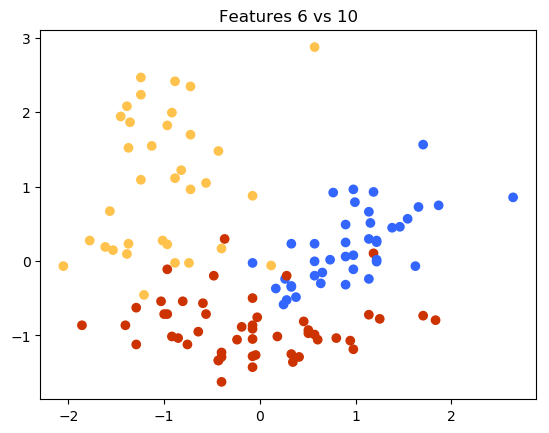
\includegraphics[scale=0.3]{img/6x10.png}&
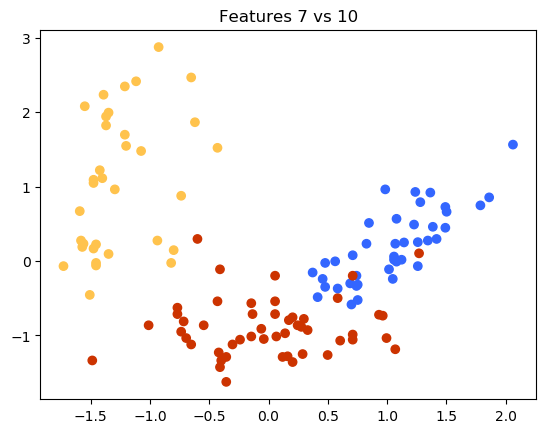
\includegraphics[scale=0.3]{img/7x10.png}&
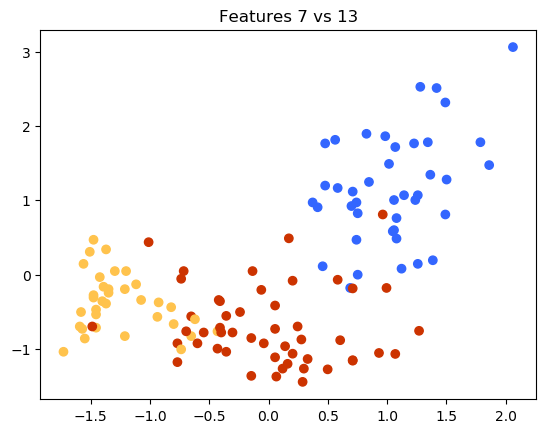
\includegraphics[scale=0.3]{img/7x13.png}&
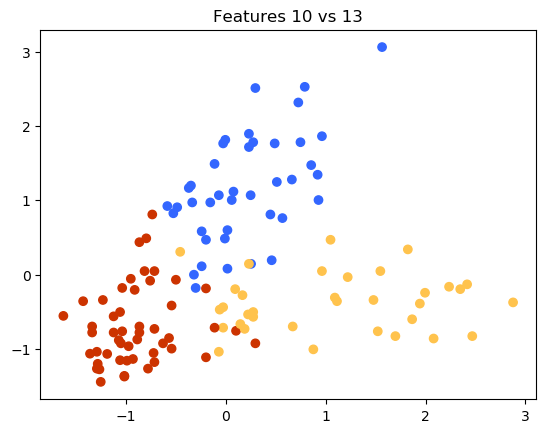
\includegraphics[scale=0.3]{img/10x13.png}
\end{tabular}
Upon further inspection we concluded that the plot of $7\ \&\ 10$ had no region where all three classes overlapped \& the class represented by yellow data points is completely distinct from the other two. Thus we decided to choose features $7\ \&\ 10$.

\section{$k$-Nearest Neighbours}
For our implementation of $k$-Nearest Neighbours we standardised the training set \& then standardised the test set using the means and variances of the training set so that the two sets were comparable. We decided that whenever a tie occurred for the dominant class we would keep discounting the furthest neighbour, until a dominant class was found. Running our implementation of $k$-Nearest Neighbours produced the confusion matrices below.
\begin{center}\begin{tabular}{ccccc}
1-Nearest Neighbour&3-Nearest Neighbour&5-Nearest Neighbour&7-Nearest Neighbour\\
\begin{tabular}{|c|c|c|}
\hline0.89&0.11&0\\
\hline0.19&0.81&0\\
\hline0&0.07&0.93\\
\hline
\end{tabular}&
\begin{tabular}{|c|c|c|}
\hline0.89&0.11&0\\
\hline0.14&0.86&0\\
\hline0&0.07&0.93\\
\hline
\end{tabular}&
\begin{tabular}{|c|c|c|}
\hline0.89&0.11&0\\
\hline0.19&0.81&0\\
\hline0&0.07&0.93\\
\hline
\end{tabular}&
\begin{tabular}{|c|c|c|}
\hline0.94&0.06&0\\
\hline0.19&0.81&0\\
\hline0&0.07&0.93\\
\hline
\end{tabular}
\end{tabular}\end{center}
The confusion matrices for $k=1,2$; $k=3,4$; and, $k=5,6$ were all the same. This is likely due, in part, to our implementation of how ties are dealt with since if ties are found for all the data points in the test set then the matrix will be the same as $k-1$. For low even values of $k$ ties are more likely.

\indent From the confusion matrices it is not clear which value of $k$ produces the best classifier since none of the matrices has a main diagonal whose values are greater than, or equal to, the values of those in the other matrices. $k=3,4$ is the best classifier for classes $2$ \& $3$; whilst $k=7$ is the best classifier for classes $1$ \& $3$. The sum of their main diagonals are both equal ($2.68$) so we cannot recommend a best value for $k$. However, if it was more important to classify class $1$ correctly, rather than class $2$, we would recommend $k=7$ and visa-versa for $k=3,4$.

\indent There is no obvious improvement in the performance of $k$-Nearest Neighbours as $k$ increases. As $k$ increases the number of neighbours to an observation being considered increases, but the influence of each neighbour decreases regardless of distance from the observation. This means that even if a test observation has the same values as a training observation it may be classified differently for $k=3$ if its next two closest neighbours are of a different class (this argument can be extended $\forall\ k>3$). This can be accounted for by weighting the influence of each neighbour inversely to its distance from the test observation, (\textit{i.e.} $\frac{1}{d}$).

\indent This issue is further exaggerated for outliers. Since few training observations have similar features to an outlier, as $k$ increases we consider observations that are highly removed from the test observation \& thus little relevance to the outlier observation.

\indent Increasing the training set size would greatly increase the quality of the $k$-Nearest Neighbours classifier as it would reduce the chance of an unfortunately place test point being classified as a different class than the one whose centre it is closest to. As the size of the training set increases the need to weight the influence of neighbours decreases as test points are more likely to be close to relevant neighbours.

\section{Alternative Classifier - Na\"ive Bayes}
We chose to implement the Na\"ive Bayes classifier since the instance space of the initial scatter plot, for features $7$ \& $10$, did not look like it could be well partitioned by axis-parallel decision boundaries, thus making a Decision Tree a bad classifier. The scatter plot does not show any apparent relationship between features $7$ \& $10$ so we assumed that they are independent, otherwise Na\"ive Bayes would not be as effective. Again we standardised all the data, as described above. Implementing a Na\"ive Bayes classifier on features $7$ \& $10$ produced the following confusion matrix.
\begin{center}\begin{tabular}{c}
Na\"ive Bayes Classifier\\
\begin{tabular}{|c|c|c|}
\hline1&0&0\\
\hline0.52&0.43&0.05\\
\hline0&0.14&0.86\\
\hline
\end{tabular}
\end{tabular}\end{center}

The confusion matrix shows us that our implementation of the \textit{Na\"ive Bayes} classifier perfect classifies data points of class $1$ as class $1$, which is better than $k$-Nearest Neighbours for all values of $k$. However, it performs significantly worse than all the $k$-Nearest Neighbours classifiers when classifying class $2$. Its performance here is notably poor as it classifiers more of the class $2$ test data as class $1$ than as class $2$. Its performance for class $3$ is worse than all the $k$-Nearest Neighbours but is still pretty good. It is hard to recommend using Na\"ive Bayes over $k$-Nearest Neighbours due to its poor classification of class $2$, but if we knew that class $1$ was significantly more likely than the other two then it may be appropriate to use Na\"ive bayes.

\indent $k$-Nearest Neighbours and Na\"ive Bayes are very different classifiers. $k$-Nearest Neighbours assumes nothing about the distribution of data, and cares solely about the relative distance between points. Whereas Na\"ive Bayes, considers the whole dataset by looking at the spread of data across all features. This enables Na\"ive Bayes to make more informed decisions as to which class test points belong to, and reduces the error made when classifying outlier points.

\indent Increasing the training set size would improve the Nai\"ve Bayes classifier, but only to a certain point as each additional data point has a decreasing influence on the variance \& mean of its cluster. However, new points closer to the centre of a cluster would drastically reduce the effect of outlier points to a classes distribution, which would create greater discrimination between the classes.

\indent Increasing the number of features being analysed by Na\"ive Bayes would improve the performance of the classifier as long as all the features are independent. If features $A$ is dependent on feature $B$ then the influence of feature $B$ on the classifier will be greater than that of the other features, which is likely to be undesirable. 

\section{Using Three Features}
We began our hunt for a third feature with a qualitative approach, using python to plot 3D scatter plots of features $7$ \& $10$ against each of the remaining $11$ features. This quickly proved difficult to interpret reliably. It was easy to identify certain plots that were clearly unsuitable (such as $7$ vs $10$ vs $11$) due to too much overlap between classes. But most plots seemed very similar \& thus choosing the best would be difficult.\\
\indent So we decided to take a quantitative approach. We calculated the multiple correlation coefficient between features $7$ \& $10$ and the $11$ other features, using the formula\footnote{src: {\ttfamily{www.real-statistics.com/correlation/multiple-correlation/}}}
$$R_{z,x,y}=\sqrt{\frac{r_{xz}^2+r_{yz}^2-2r_{xz}r_{yz}r_{xy}}{1-r_{xy}^2}}$$
where $r_{xy}$ is the correlation coefficient for features $x$ \& $y$. This produced the following results
\begin{center}
\begin{tabular}{|c|c|c|c|c|c|c|c|}
\hline i&$R_{i,7,10}$&i&$R_{i,7,10}$&i&$R_{i,7,10}$&i&$R_{i,7,10}$\\
\hline 1&0.692&4&0.380&8&0.550&12&0.852\\
2&0.408&5&0.378&9&0.683&13&0.852\\\cline{7-8}
3&0.348&6&0.868&11&0.738\\\cline{1-6}
\end{tabular}
\end{center}
This shows that feature $6$ has the greatest correlation with features $7$ \& $10$, so we chose to proceed with feature $6$. We implemented a $k$-Nearest Neighbours Classifier for features $6,7\ \& 10$, standardising all the data as before. This produced the following confusion matrices
\begin{center}\begin{tabular}{ccccc}
1-Nearest Neighbour&3-Nearest Neighbour&5-Nearest Neighbour&7-Nearest Neighbour\\
\begin{tabular}{|c|c|c|}
\hline1&0&0\\
\hline0.19&0.81&0\\
\hline0&0.07&0.93\\
\hline
\end{tabular}&
\begin{tabular}{|c|c|c|}
\hline1&0&0\\
\hline0.19&0.81&0\\
\hline0&0.07&0.93\\
\hline
\end{tabular}&
\begin{tabular}{|c|c|c|}
\hline1&0&0\\
\hline0.19&0.81&0\\
\hline0&0.07&0.93\\
\hline
\end{tabular}&
\begin{tabular}{|c|c|c|}
\hline1&0&0\\
\hline0.19&0.81&0\\
\hline0&0.07&0.93\\
\hline
\end{tabular}
\end{tabular}\end{center}
It is notable that the confusion matrices are the same for all values of $k$. This is due to the neighbourhood of a point vanishing as dimensionality increases, decreasing the influence of points. We may have points which are very close in value for two features, but drastically different for the third \& thus would not be classed as neighbours (for low $k$).

\indent Using three features resulted in a perfect classification of class $1$, which was not achieved by using just two features (for any values of $k$) but was achieved by our Na\"ive Bayes classifier. Using just two features resulted in a better classifier of class $2$, when $k=3,4$. Using either two \& three features results in the same performance when classifying class $3$. Since the sum of the main diagonal for using three features is $2.74$, which is strictly greater than that when using two features we deem the three feature classifier to be better. However if classifying class $2$ correctly is more important than classifying class $1$ correctly then two features is better.

\indent Increasing the complexity of our classifier has reduced our sample density within the sample space. Lower sample density makes it easier to partition the sample space into linearly separable class-homogeneous regions since the chance of a sample lying outside its class region has decreased. This means we are more likely to produce regions that include outliers since it is easier to attach them to a region, this results in overfitting of the data. Although there is no apparent evidence for overfitting of the data in this particular instance this may be due to the relatively small testing set. We would not recommend increasing the number of features any further as this would increase the likelihood of overfitting \& thus a worse classifier.

\section{Principal Component Analysis}
Using Scipy's PCA object we fitted \& transformed the training data to produce the following plot.
\begin{center}
\begin{tabular}{cc}
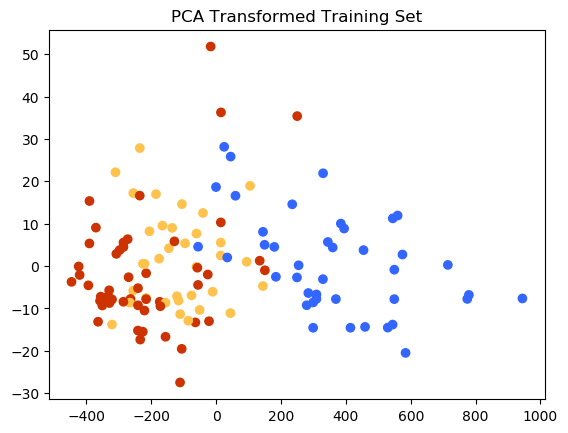
\includegraphics[scale=0.3]{img/pca.png}&
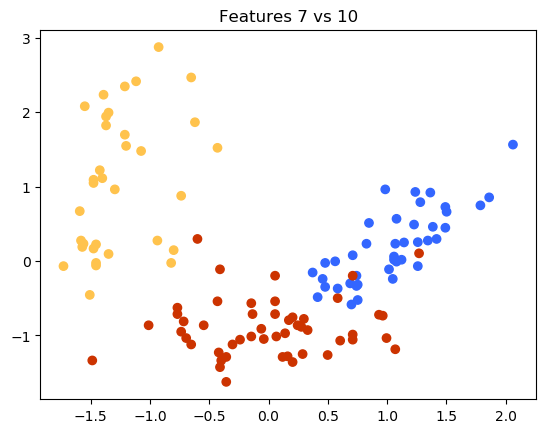
\includegraphics[scale=0.3]{img/7x10.png}
\end{tabular}
\end{center}
The PCA plot appears to be much worse than that of our manually selected features, due to the class-clusters being less distinct. Notably, the difference of the scales of the axes is much greater in the PCA plot meaning the feature describe by the vertical axis will have a greater effect on the distance function value.\\
\indent Using the $k$-Nearest Neighbours classifier with the transformed training \& test sets produced the following confusion matrix
\begin{center}\begin{tabular}{ccccc}
1-Nearest Neighbour&3-Nearest Neighbour&5-Nearest Neighbour&7-Nearest Neighbour\\
\begin{tabular}{|c|c|c|}
\hline0.83&0&0.17\\
\hline0.05&0.57&0.38\\
\hline0.07&0.14&0.79\\
\hline
\end{tabular}&
\begin{tabular}{|c|c|c|}
\hline0.83&0&0.17\\
\hline0.10&0.62&0.28\\
\hline0.07&0.36&0.57\\
\hline
\end{tabular}&
\begin{tabular}{|c|c|c|}
\hline0.83&0&0.17\\
\hline0.05&0.67&0.28\\
\hline0&0.21&0.79\\
\hline
\end{tabular}&
\begin{tabular}{|c|c|c|}
\hline0.89&0&0.11\\
\hline0.05&0.62&0.33\\
\hline0&0.15&0.86\\
\hline
\end{tabular}
\end{tabular}\end{center}
From these confusion matrices $k=7$ appears to be the best classifier as it has the greatest accuracy for classes $1$ \& $3$, however $k=5$ has the greatest accuracy for class $2$ (although it still performs poorly). There is no apparent increase in accuracy as $k$ increases since $k=1$ is strictly more accurate than $k=3$, but strictly less than $k=7$.

\indent Comparing these results to the classifier using our two manually chosen features, the manually chosen classifier is strictly more accurate for every class. This is likely due to PCA only being highly effective at very large dimensions of data (\textit{e.g.} $d>1000$). Here we have only 13 dimensions which is relatively low. At very high dimensions it becomes impractical to perform qualitative analysis for feature selection \& thus PCA becomes useful. PCA is good at reducing noise in a data set, the fact that this has not improved the classifier suggests that our data set has relatively low noise. PCA does not account for class labels when transforming data, rather it tries to find underlying relationships between features which is hard to do at low dimensionality. When we manually chose our features we did account for classes \& thus would expect a greater accuracy.

\subsection*{Conclusion}
We consistently standardised all the data we were analysing (except with PCA where SciPy does), this will have caused a fundamental change in the performance of our classifiers but should result in a greater accuracy. We can always adjust how we standardise the data in order to further improve performance, likely using a trial-and-improvement approach.

\indent From all the classifiers we used the $k$-Nearest Neighbour classifiers with manually selected features were the most accurate. This is likely due to the low dimensionality of the data sets which mean that the qualitative analysis we did is likely to outperform any quantitative approaches. With a greater understanding about the composition of wine we may be able to extract more features for the initial $13$, making the qualitative approach of PCA more viable. But it is equally likely that this would improve our quantitative analysis due to greater prior knowledge.

\end{document}